\documentclass[t,xcolor={usenames,dvipsnames}]{beamer}

\mode<presentation>
{
\usetheme{Frankfurt}%{Warsaw}
%\setbeamercovered{transparent}
%\setbeamercolor{background canvas}{bg=white}
}

% Delete these, if you do not want the table of contents to pop up at
% the beginning of each (sub)section:
%\AtBeginSubsection[]
%{
%  \begin{frame}<beamer>{Outline}
%    \tableofcontents[currentsection,currentsubsection]
%  \end{frame}
%}
%\AtBeginSection[]
%{
%  \begin{frame}<beamer>{Outline}
%    \tableofcontents[currentsection]
%  \end{frame}
%}

\usepackage[english]{babel}
\usepackage[latin1]{inputenc}
\usepackage{times}
\usepackage[T1]{fontenc}
\usepackage{verbatim}
\usepackage{url}
\usepackage{amsmath,amssymb}
\usepackage{comment}
\usepackage[overlay,absolute]{textpos}
\usepackage{hyperref}

% Author-date citations
\usepackage[authoryear,round]{natbib}
\let\cite=\citep  % default \cite such as {\LaTeX} authors are used to

% Where \includegraphics should look for figures
\graphicspath{{./figs/}{../group_talk_2011_11_29/figs/}}
\usepackage{epstopdf}
\DeclareGraphicsExtensions{.eps,.png,.jpg,.pdf}

% Shortcuts
\newcommand{\myhref}[2]{\href{#1}{\textcolor{Blue}{#2}}}
\newcommand{\myurl}[1]{\myhref{#1}{#1}}
\newcommand{\subitem}[1]{\begin{itemize}[<.->]\item #1 \end{itemize}}
\newcommand{\ghead}[1]{{\tiny #1\\}}
\newcommand{\doi}[1]{\myhref{http://dx.doi.org/#1}{doi:#1}}
\newcommand{\csym}[1]{\textcolor{Blue}{\texttt{#1}}}
\newcommand{\ud}{\mathrm{d}}
\newcommand{\dt}{\ud t}

%%%%%%%%%%%%%%%%%%%%%%%%%%%%%%%%%%%%%%%%%%%%%%%%%%%%%%%%%%%%%%%%%%%%%%
\title{Functional Curation of Mathematical Models}
\author{Jonathan Cooper}
\institute[University of Oxford]
{Computational Biology Group\\
 Department of Computer Science\\
 University of Oxford}
\date{December 4, 2013}

\begin{document}

\begin{frame}
\titlepage
\end{frame}

\begin{comment}
Abstract:
How do we determine if a mathematical model of a biological system is useful for a particular study? Given multiple models of a system, representing different hypotheses, how do we choose between them?  This talk will introduce a computational framework for addressing such questions.

Audience have an academic background in Biology, Biochemistry or Chemistry and have completed the DTC's 2 week introductory mathematics course. Aim to provide an introduction to the role and applications of mathematical, computational and systems biology approaches in biological research.

Duration: 40 mins
 - refer back to Gary's talk
   - ion channel screens as example expt in motivation
\end{comment}

%%%%%%%%%%%%%%%%%%%%%%%%%%%%%%%%%%%%%%%%%%%%%%%%%%%%%%%%%%%%%%%%%%%%%%

\begin{frame}{Outline}
\setcounter{tocdepth}{1}
\tableofcontents
\end{frame}

%%%%%%%%%%%%%%%%%%%%%%%%%%%%%%%%%%%%%%%%%%%%%%%%%%%%%%%%%%%%%%%%%%%%%%
\section{Motivation}
\subsection*{Main}
%%%%%%%%%%%%%%%%%%%%%%%%%%%%%%%%%%%%%%%%%%%%%%%%%%%%%%%%%%%%%%%%%%%%%%

\begin{frame}{Modelling biology}
\begin{itemize}[<+->]
\item A mathematical model encodes a quantitative hypothesis about a biological system
\item It can be used to make predictions about the response of the system to experiments
  \subitem{``If I make this intervention, I expect to see that change''}
\item Increasingly, models build on previously published models
  \begin{itemize}
  \item Compose models together to study larger system
    % examples: reaction networks, nephrons/kidneys, heart
  \item Extend or modify models to incorporate latest understanding, or look at effect of disease / drug / species / age / \ldots
  \end{itemize}
\end{itemize}
\end{frame}


\begin{frame}{Using models}
\begin{itemize}[<+->]
\item As hypothesis encodings, models are developed \emph{for a specific purpose}
  \subitem{May not be appropriate for studying same system in different context}
\item How can we\ldots
  \begin{itemize}
  \item determine a model's functionality, i.e.\ its suitability or limitations for a new study?
  \item re-use a model in a different experimental context?
  \item compare hypotheses: different models' behaviours under the same experiment?
  \end{itemize}
\end{itemize}
\end{frame}


\begin{frame}{Models and experiments}
\small
Suppose we have our mathematical model, e.g.\ Hund \& Rudy 2004:\\
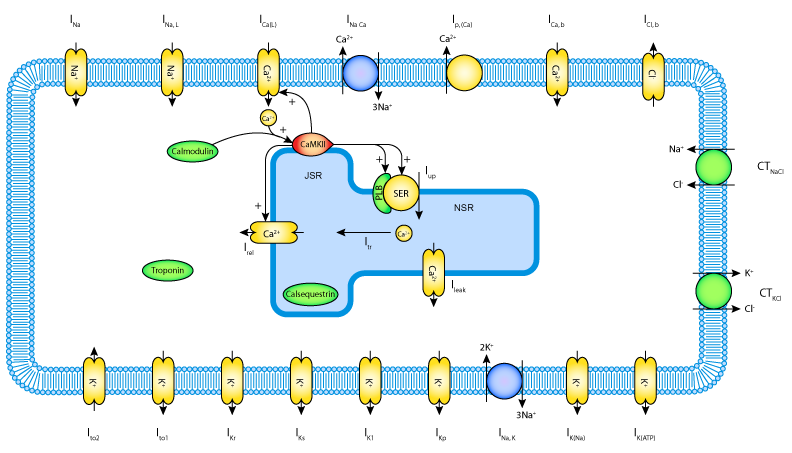
\includegraphics[width=\textwidth]{hund_2004}\\
We want to perform various potentially complex interventions\ldots
\end{frame}


\begin{frame}{Experiment: $I_{\textrm{Ca}_L}$ voltage clamp}
\begin{center}
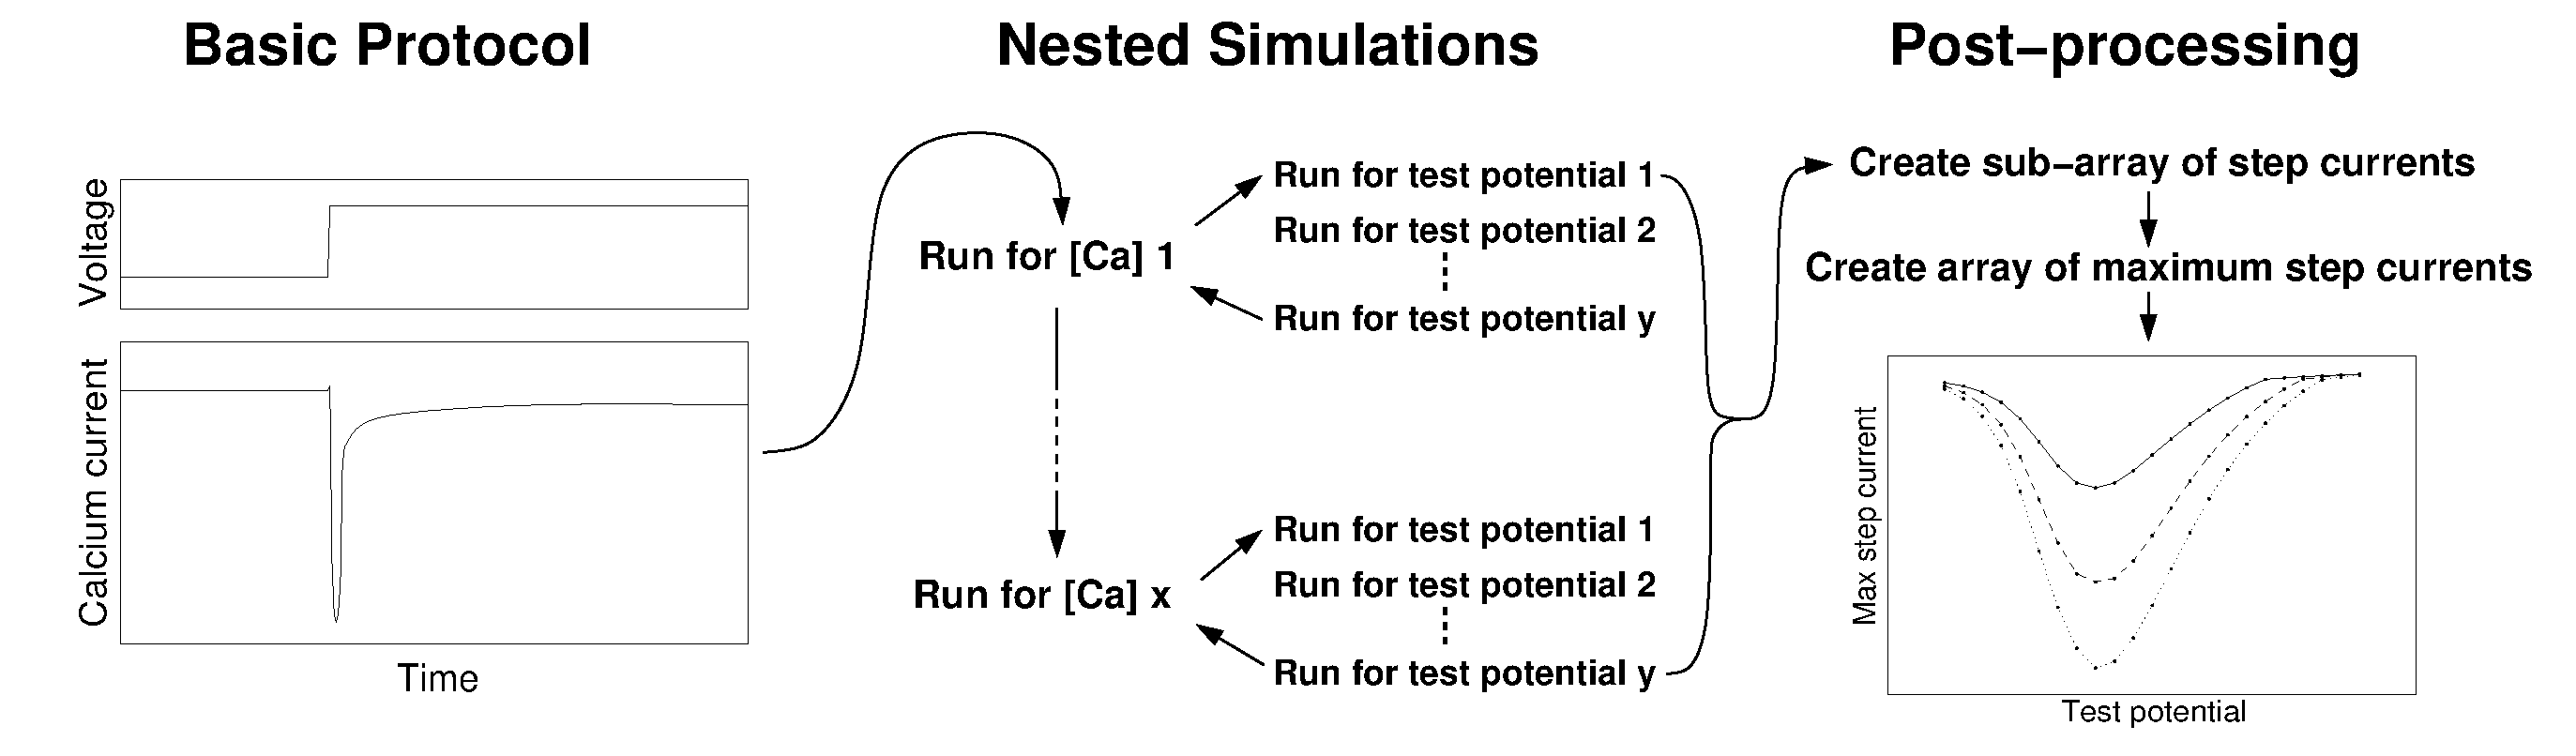
\includegraphics[width=\textwidth]{ICaLIntro}
\end{center}
%Used for ion channel screens by pharma, c.f. Gary's talk
\end{frame}


\begin{frame}{Experiment: S1-S2 restitution}
\begin{center}
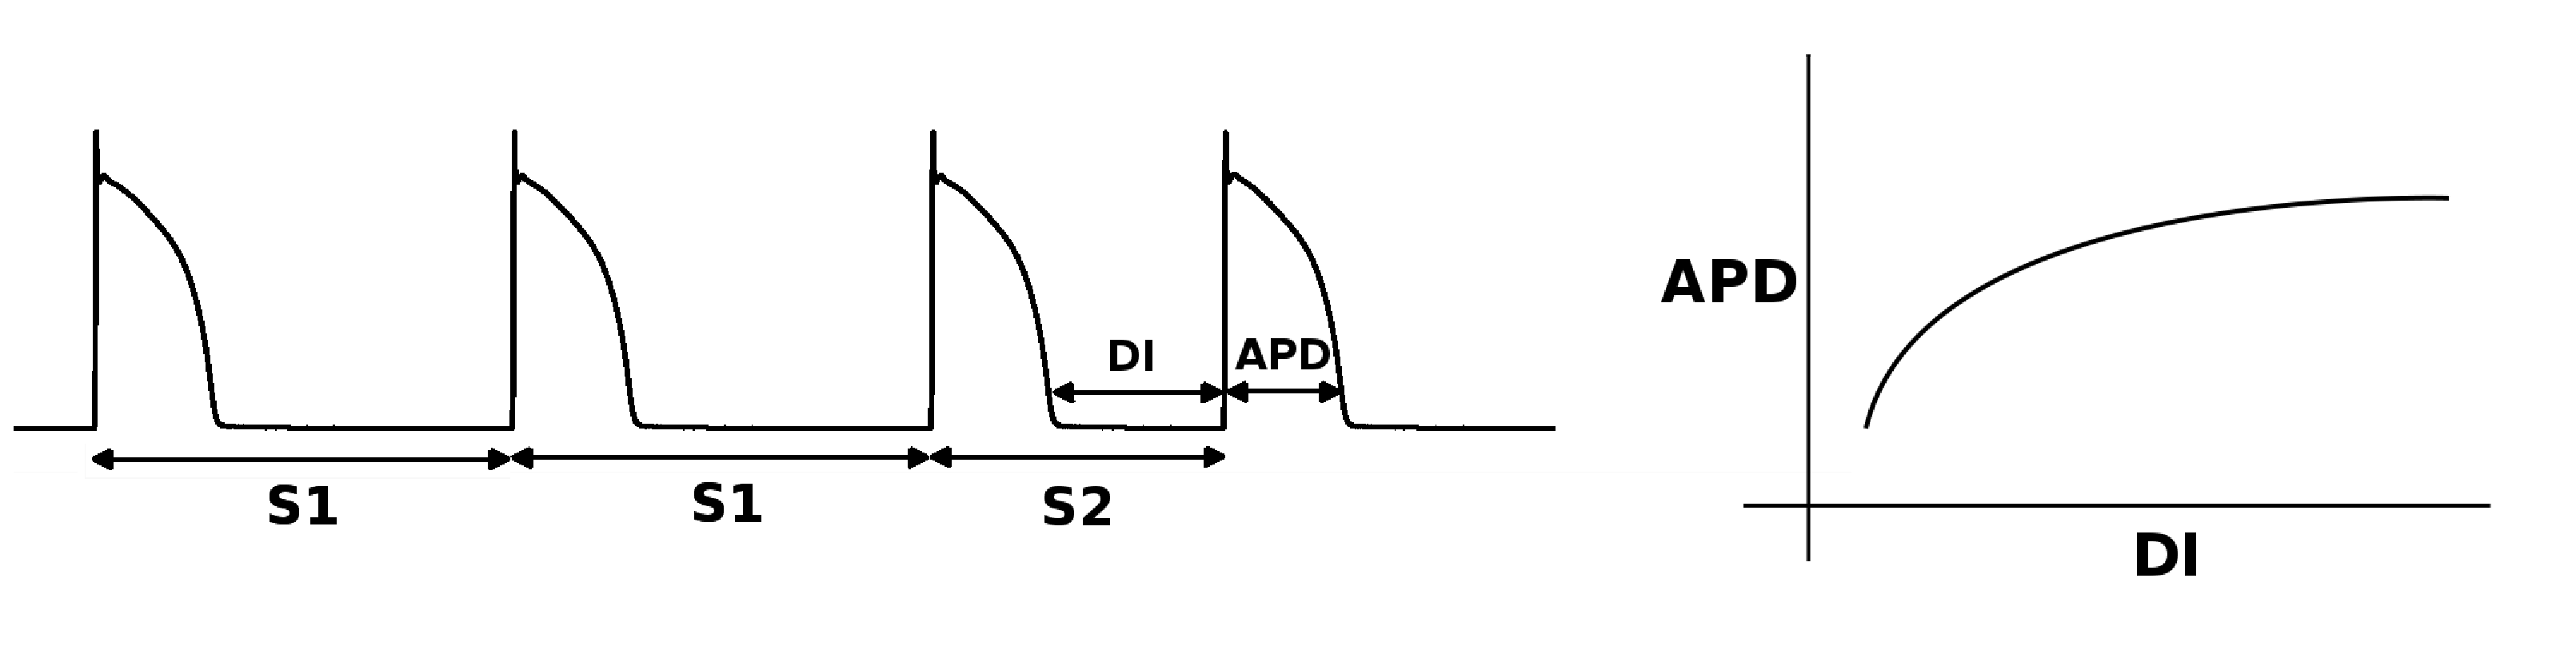
\includegraphics[width=\textwidth]{S1S2}
\end{center}
\end{frame}


%%%%%%%%%%%%%%%%%%%%%%%%%%%%%%%%%%%%%%%%%%%%%%%%%%%%%%%%%%%%%%%%%%%%%%
\section{Functional curation with virtual experiments}
\subsection*{Main}
%%%%%%%%%%%%%%%%%%%%%%%%%%%%%%%%%%%%%%%%%%%%%%%%%%%%%%%%%%%%%%%%%%%%%%

\begin{frame}{The essence}
\subitem{Separate \alert{model structure} and \alert{experimental scenario}}
\begin{center}
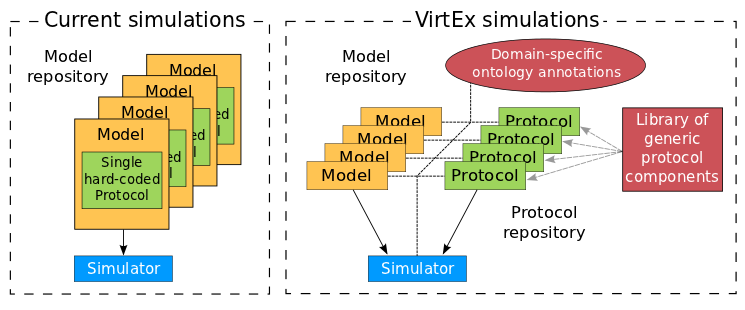
\includegraphics[width=.9\textwidth]{VirtEx_overview}
\end{center}
\vspace{-.25cm}
\begin{itemize}
\item Apply any \alert{virtual experiment} to any (relevant) model
\item One definitive version of each model / protocol
\item Automatically generate post-processed outputs, plots, etc.
\end{itemize}
\end{frame}


\begin{frame}{Foundations: a mosaic of standards}
\begin{center}
\includegraphics<1->[scale=.5]{standards_mosaic}\\
{\tiny Fig.: Mosaic of standards, adapted from (\textit{Chelliah et al., 2009, DILS})}
\end{center}
\end{frame}

\begin{frame}{Foundations: a mosaic of standards}
\begin{center}
\includegraphics<1->[scale=.5]{standards_mosaic}\\
{\tiny Fig.: Mosaic of standards, adapted from (\textit{Chelliah et al., 2009, DILS})}
\end{center}
\TPGrid{2}{2}
\begin{textblock}{2}[0.5,0.5](1,1.2)
\centering

\includegraphics[scale=.8]{COMBINE}
\end{textblock}
\end{frame}


\begin{frame}{What goes in a protocol?}
\begin{itemize}
\item Definition of the interface with the model being experimented on
  \begin{itemize}
  \item Handle variations in modelling conventions: naming, encoding the biology in mathematics
  \item Isolate sub-models, using inputs \& outputs of interest
  \end{itemize}
\item Definition of simulations to perform
\item Post-processing operations on simulation results
\item Description of what to plot
\end{itemize}
\end{frame}


\begin{frame}{Simulation Experiment Description Markup Language}
\begin{center}
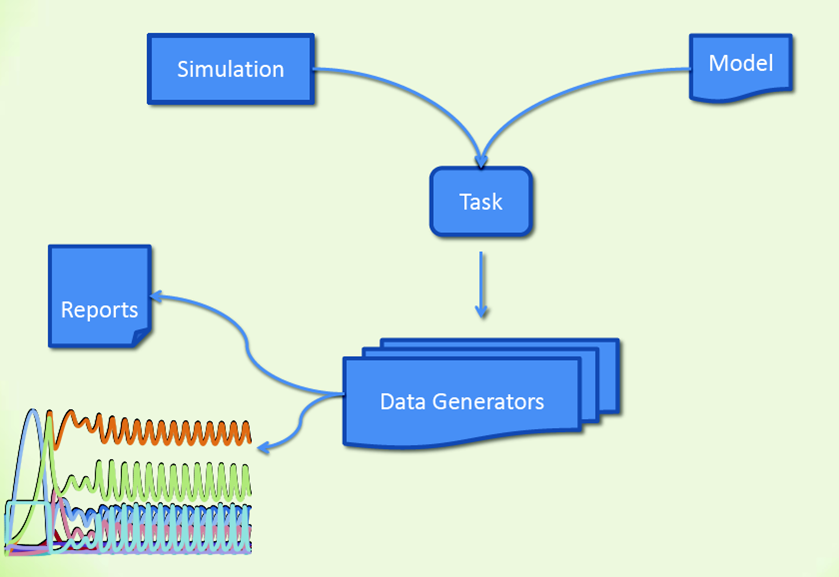
\includegraphics[scale=.5]{SEDML_overview}\\
{\tiny Fig.: SED-ML structure. \textit{Waltemath et al., BMC Sys Biol (2011)}}
\end{center}
\end{frame}


\begin{frame}{Our protocol structure}
\begin{center}
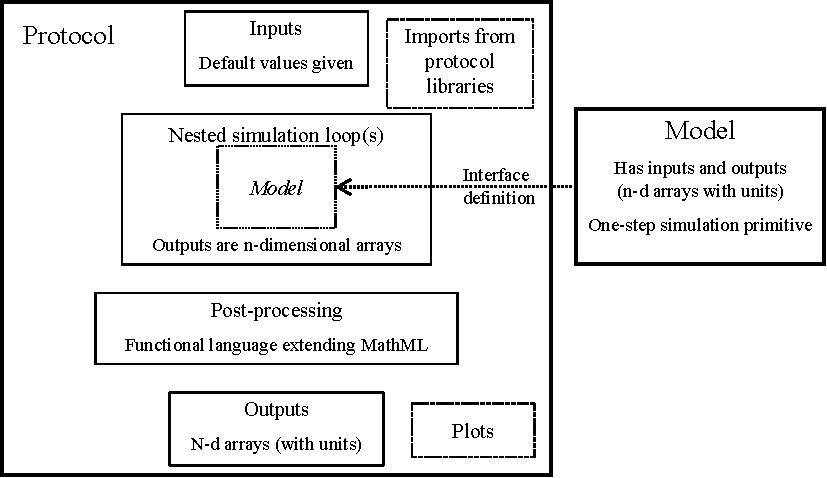
\includegraphics[width=\textwidth]{protocol_language}
\end{center}
\end{frame}


%%%%%%%%%%%%%%%%%%%%%%%%%%%%%%%%%%%%%%%%%%%%%%%%%%%%%%%%%%%%%%%%%%%%%%
\section{Examples}
%%%%%%%%%%%%%%%%%%%%%%%%%%%%%%%%%%%%%%%%%%%%%%%%%%%%%%%%%%%%%%%%%%%%%%

\subsection*{S1-S2}
%%%%%%%%%%%%%%%%%%%

\begin{frame}{Example: S1-S2 restitution}
\begin{center}
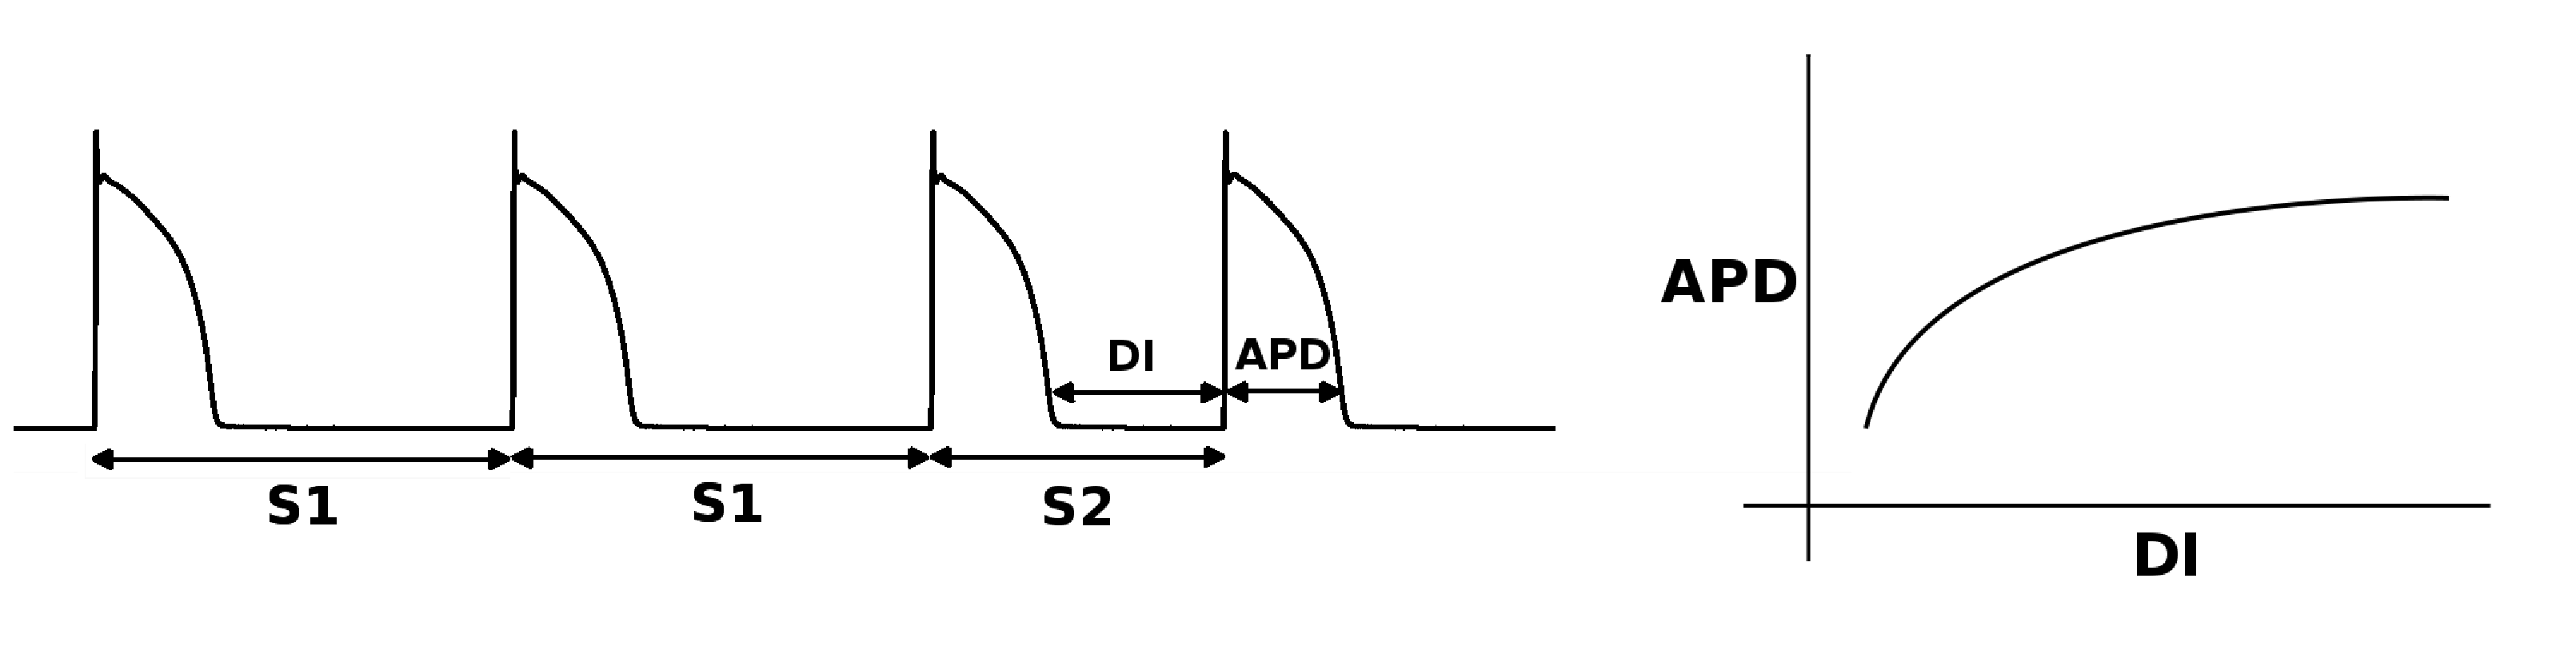
\includegraphics[width=\textwidth]{S1S2}
\end{center}
\end{frame}

\begin{frame}{Example: S1-S2 restitution on canine models}
\begin{columns}[T]
\begin{column}{.33\linewidth}
\begin{center}
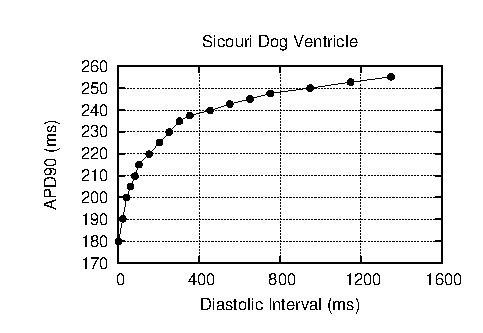
\includegraphics[width=\textwidth]{sicouri_dog_ventricle_s1s2_curve}\\
\vspace{.1cm}
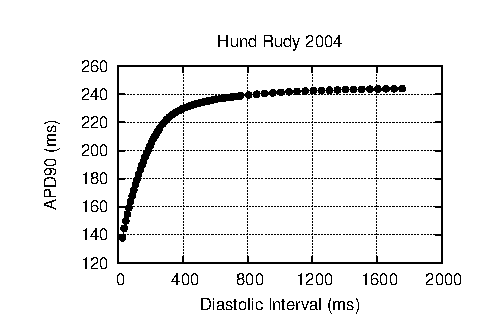
\includegraphics[width=\textwidth]{hund_rudy_2004_s1s2_curve}
\end{center}
\end{column}
\begin{column}{.33\linewidth}
\begin{center}
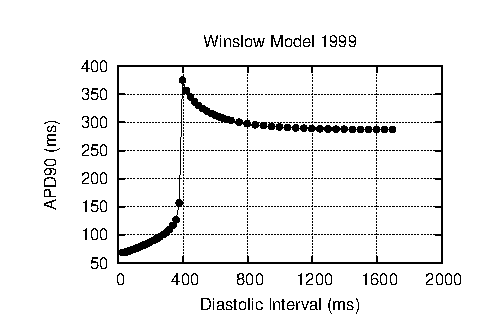
\includegraphics[width=\textwidth]{winslow_model_1999_s1s2_curve}\\
\vspace{.1cm}
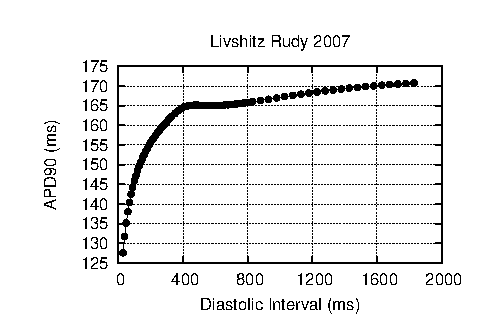
\includegraphics[width=\textwidth]{livshitz_rudy_2007_s1s2_curve}
\end{center}
\end{column}
\begin{column}{.33\linewidth}
\begin{center}
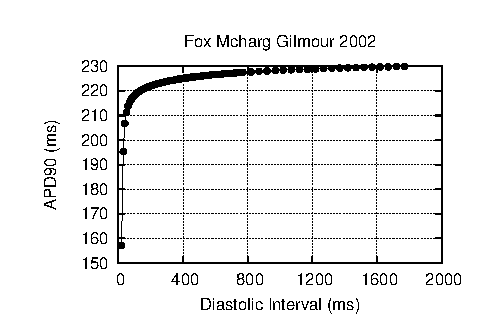
\includegraphics[width=\textwidth]{fox_mcharg_gilmour_2002_s1s2_curve}\\
\vspace{.1cm}
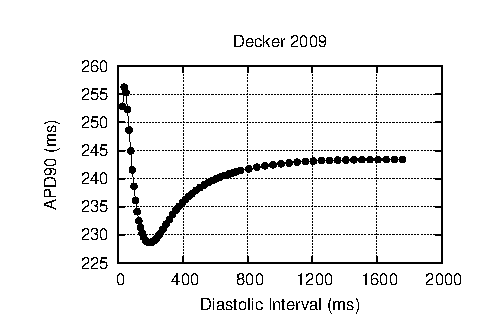
\includegraphics[width=\textwidth]{decker_2009_s1s2_curve}
\end{center}
\end{column}
\end{columns}
\end{frame}


\begin{frame}{Example: S1-S2 restitution on human models}
\begin{columns}[T]
\begin{column}{.33\linewidth}
\begin{center}
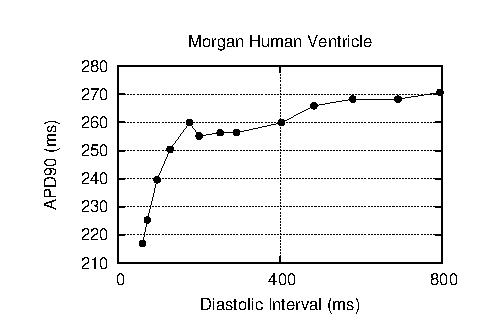
\includegraphics[width=\textwidth]{morgan_human_ventricle_s1s2_curve}\\
\vspace{.1cm}
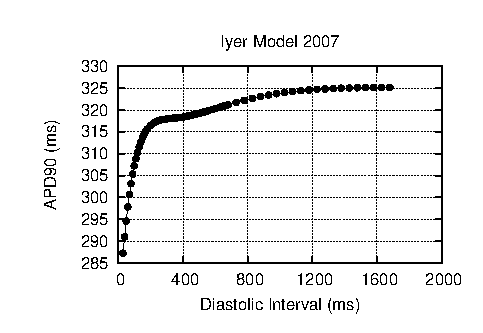
\includegraphics[width=\textwidth]{iyer_model_2007_s1s2_curve}
\end{center}
\end{column}
\begin{column}{.33\linewidth}
\begin{center}
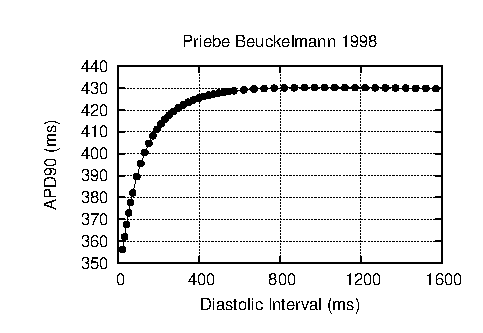
\includegraphics[width=\textwidth]{priebe_beuckelmann_1998_s1s2_curve}\\
\vspace{.1cm}
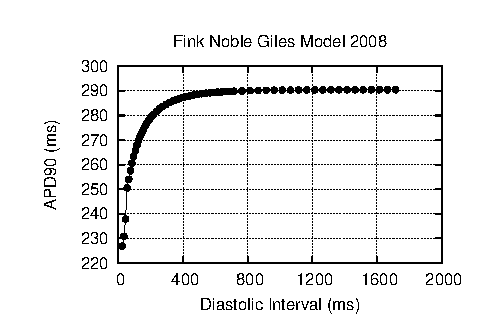
\includegraphics[width=\textwidth]{fink_noble_giles_model_2008_s1s2_curve}
\end{center}
\end{column}
\begin{column}{.33\linewidth}
\begin{center}
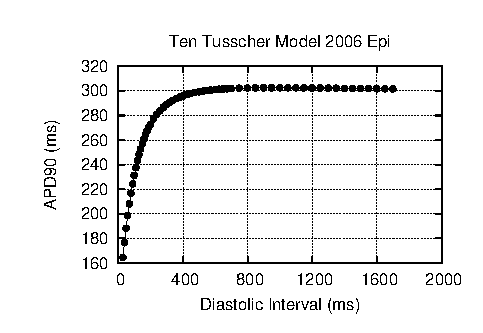
\includegraphics[width=\textwidth]{ten_tusscher_model_2006_epi_s1s2_curve}\\
\vspace{.1cm}
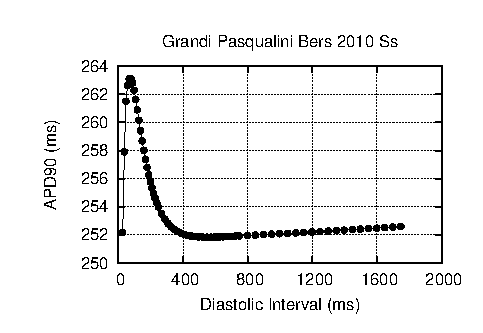
\includegraphics[width=\textwidth]{grandi_pasqualini_bers_2010_ss_s1s2_curve}
\end{center}
\end{column}
\end{columns}
\end{frame}


\begin{frame}{Challenges in APD calculation}
\begin{center}
\includegraphics<1>{faber_rudy_2000_s1s2_curve}
\only<2>{\vspace{-.5cm}}
\includegraphics<2>[height=.9\textheight]{faber_rudy_2000_COR_comparison}
\end{center}
\end{frame}


\subsection*{ICaL}
%%%%%%%%%%%%%%%%%%

\begin{frame}{Example: $I_{\textrm{Ca}_L}$ voltage clamp}
\begin{center}
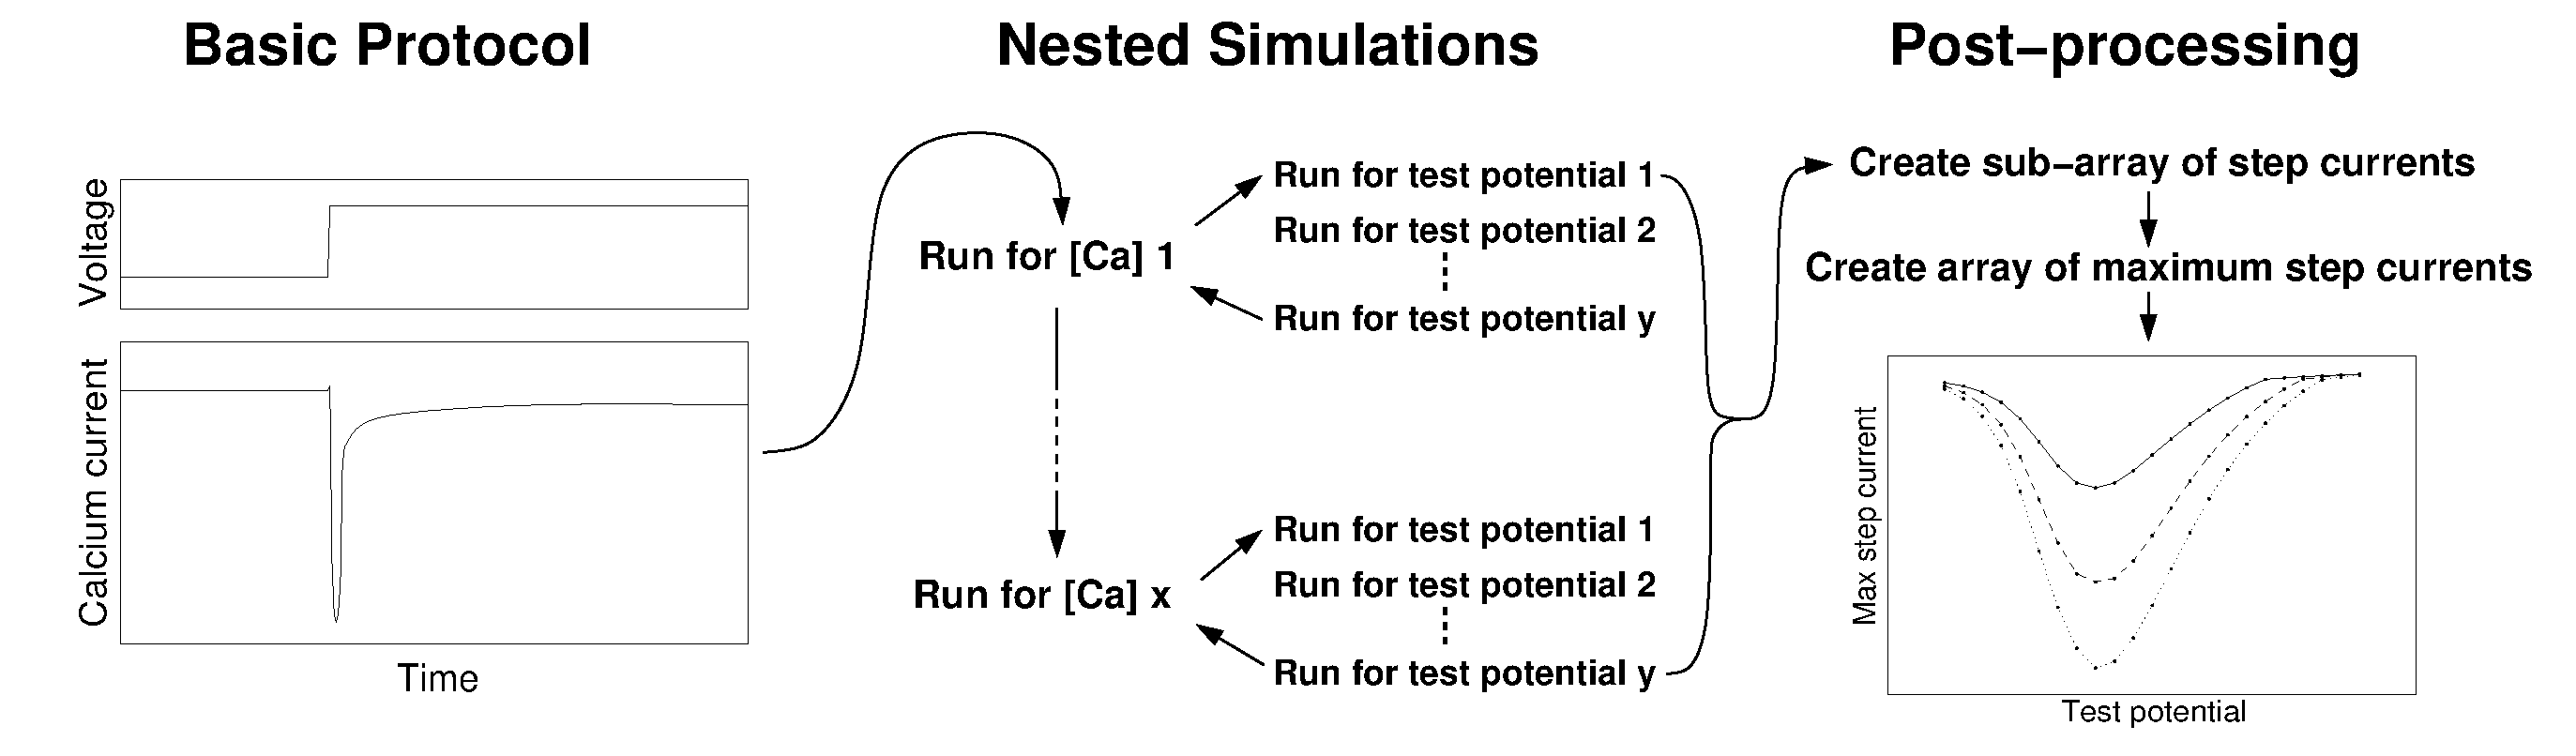
\includegraphics[width=\textwidth]{ICaLIntro}
\end{center}
\end{frame}

\begin{frame}{Example: $I_{\textrm{Ca}_L}$ voltage clamp}
\begin{columns}[T]
\begin{column}{.33\linewidth}
\begin{center}
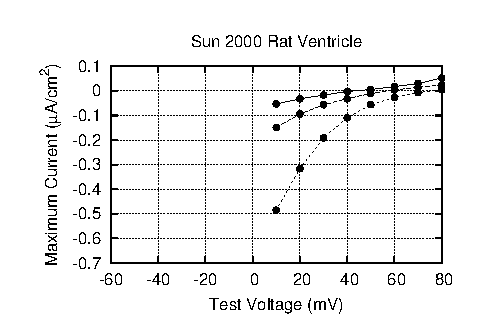
\includegraphics[width=\textwidth]{sun_rat_ventricle_ICaL_IV_curve}\\
\vspace{.1cm}
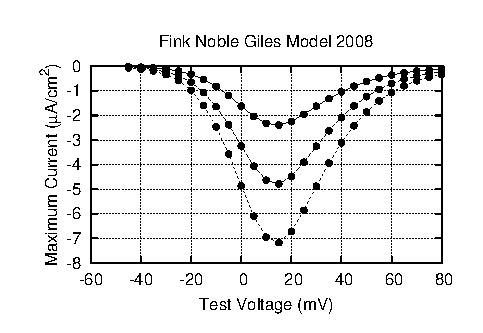
\includegraphics[width=\textwidth]{fink_noble_giles_model_2008_ICaL_IV_curve}
\end{center}
\end{column}
\begin{column}{.33\linewidth}
\begin{center}
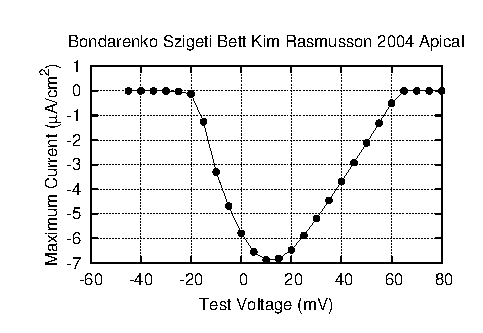
\includegraphics[width=\textwidth]{bondarenko_szigeti_bett_kim_rasmusson_2004_apical_ICaL_IV_curve}\\
\vspace{.1cm}
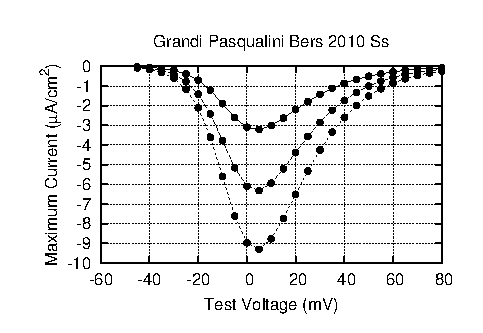
\includegraphics[width=\textwidth]{grandi_pasqualini_bers_2010_ss_ICaL_IV_curve}
\end{center}
\end{column}
\begin{column}{.33\linewidth}
\begin{center}
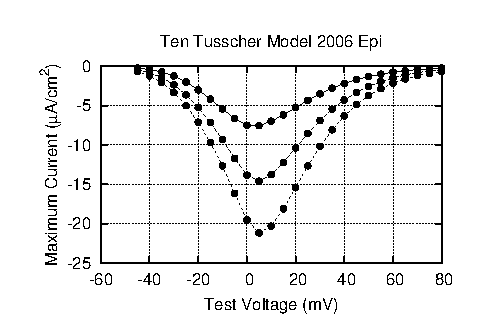
\includegraphics[width=\textwidth]{ten_tusscher_model_2006_epi_ICaL_IV_curve}\\
\vspace{.1cm}
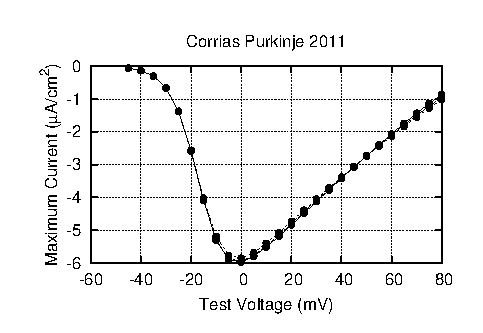
\includegraphics[width=\textwidth]{corrias_purkinje_2011_ICaL_IV_curve}
\end{center}
\end{column}
\end{columns}
\end{frame}
% Refer back to Gary's talk and IC50 calculation


\subsection*{Cell-based Chaste}
%%%%%%%%%%%%%%%%%%%%%%%%%%%%%%%

\begin{frame}{Intestinal crypts}
\begin{itemize}
\item Here a `model' is a cell-based \alert{simulation}, not just equations
  \subitem{Implemented using the cell-based functionality in Chaste}
\item Model parameters may be set
\item Execution may be nested in outer loops, e.g.\ for parameter sweep
\item Result post-processing may be performed
\end{itemize}
\end{frame}


\begin{frame}{Case study}
\centering
\begin{minipage}{0.28\textwidth}
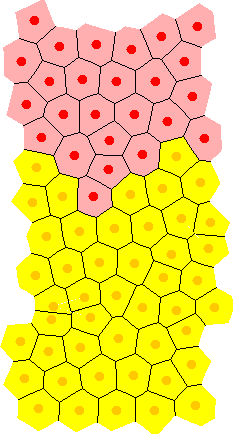
\includegraphics[width=.9\textwidth]{VariableWnt}
\end{minipage}
\begin{minipage}{0.39\textwidth}
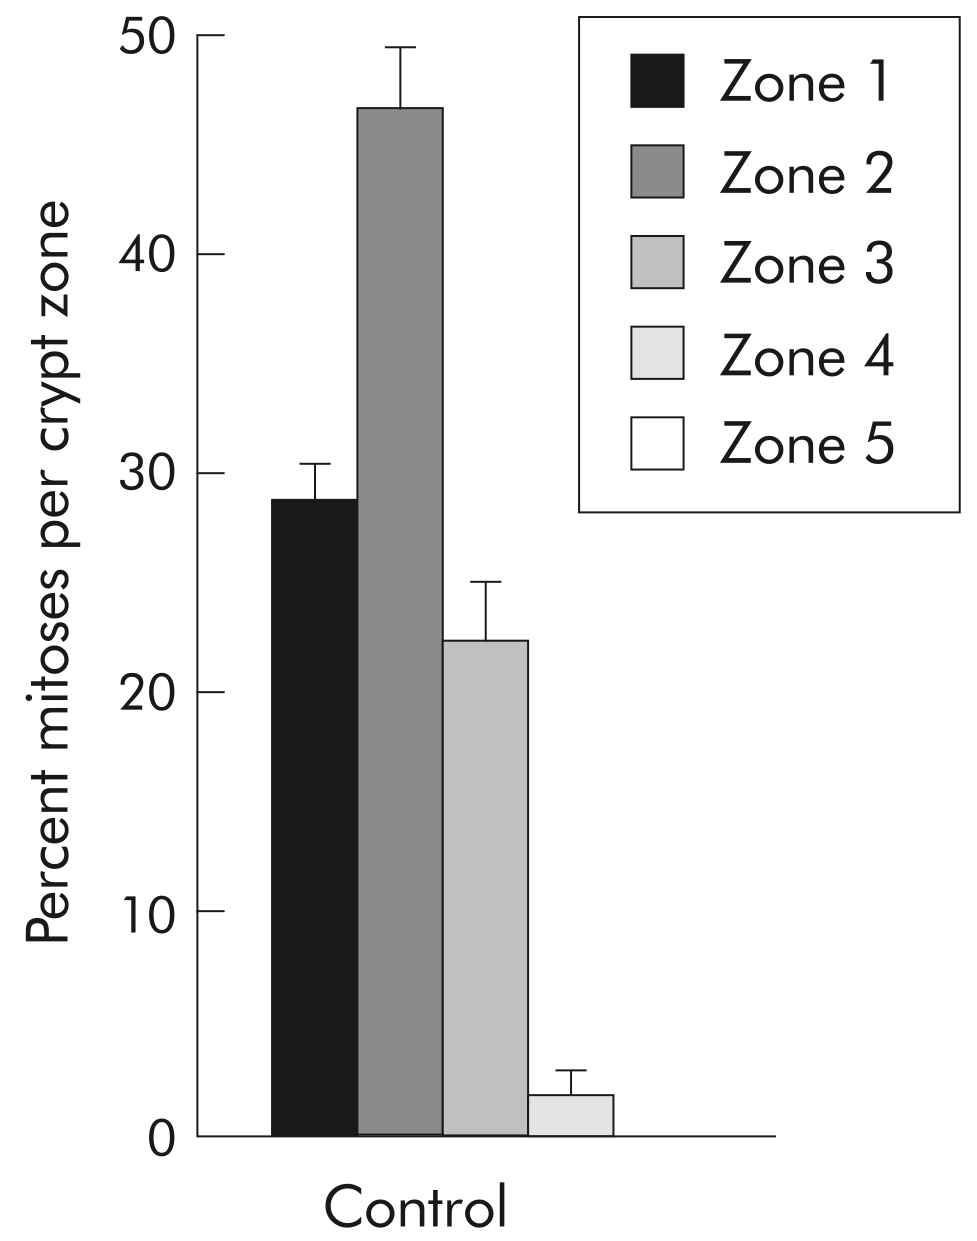
\includegraphics[width=.9\textwidth]{WongFigure}
\end{minipage}
\begin{minipage}{0.31\textwidth}
\begin{itemize}
\item Cell division locations in intestinal crypt
\item Compare three submodels for cell cycle
\item Parameter sweep over crypt height
\end{itemize}
\end{minipage}
\vspace{.4cm}
\begin{center}
\tiny
\myhref{http://dx.doi.org/10.1016/j.procs.2013.05.235}{Cooper and Osborne, ICCS 2013}
\end{center}
\end{frame}


\begin{frame}{Results}
\vspace{-.45cm}
{\footnotesize Distributions of crypt cell division events with different cell cycle models}
\vspace{-.1cm}
\hspace*{2mm}
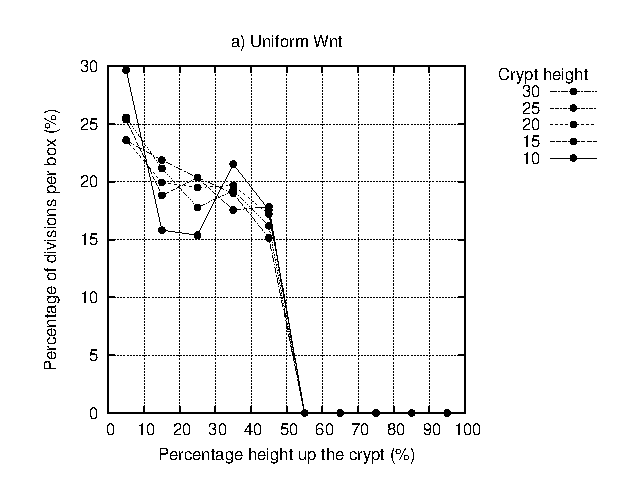
\includegraphics[width=.45\textwidth]{Uniform_Wnt-Cell_division_locations}
\hspace*{5mm}
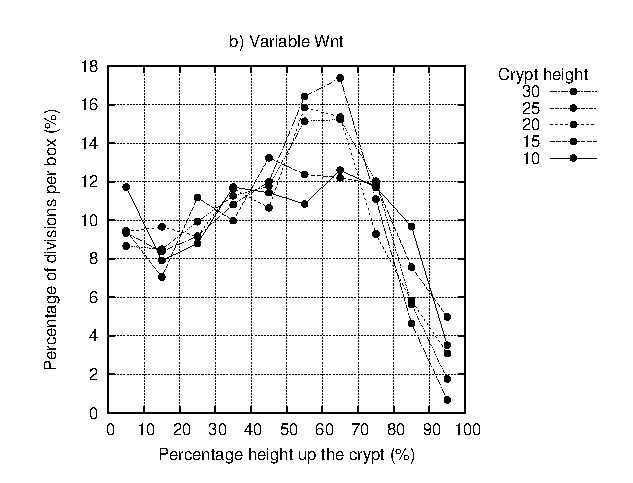
\includegraphics[width=.45\textwidth]{Variable_Wnt-Cell_division_locations}\\
\hspace*{2mm}
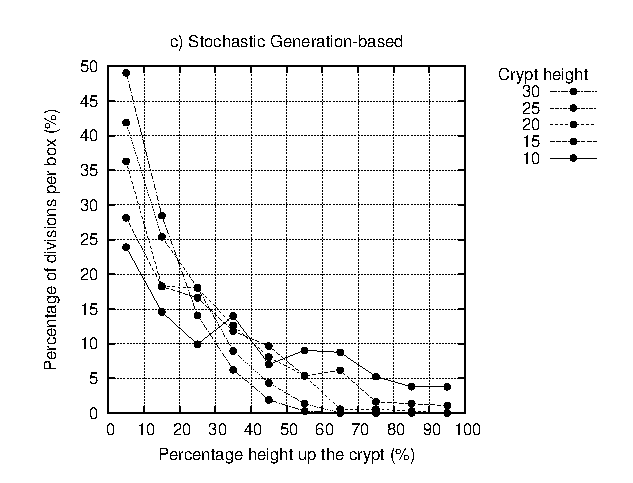
\includegraphics[width=.45\textwidth]{Stochastic_Generation-based-Cell_division_locations}
\hspace*{12mm}
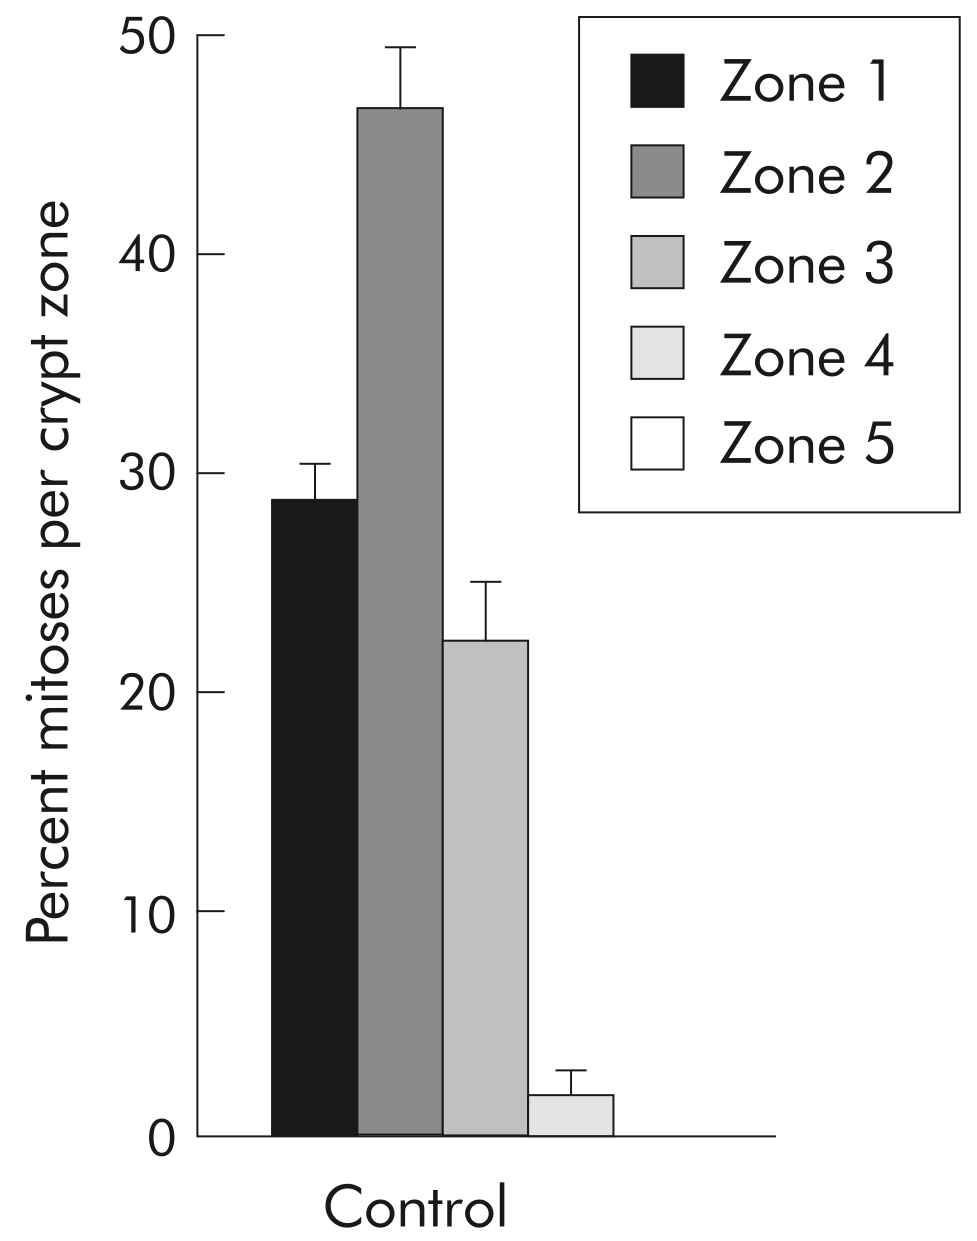
\includegraphics[height=.4\textheight]{WongFigure}
\end{frame}


\begin{frame}{Challenges arising}
\begin{itemize}[<+->]
\item Setting `biological' parameters that don't have direct representations in all models
\item Describing the coupling of component models
\item Cell birth \& death imply non-regular result arrays
  \subitem{Increases technical complexity of post-processing}
\item What post-processing should be in the protocol language?
  \begin{itemize}[<.->]
  \item What is best as dedicated code or workflow?
  \item A language targeted at protocol exchange should be supportable by multiple tools
  \item Contrast: rapid prototyping, or deposition in a repository of standard experiments
  \end{itemize}
\end{itemize}
\end{frame}


%%%%%%%%%%%%%%%%%%%%%%%%%%%%%%%%%%%%%%%%%%%%%%%%%%%%%%%%%%%%%%%%%%%%%%
\section{Conclusions and future directions}
\subsection*{Main}
%%%%%%%%%%%%%%%%%%%%%%%%%%%%%%%%%%%%%%%%%%%%%%%%%%%%%%%%%%%%%%%%%%%%%%

\begin{frame}{Goals of this work}
\begin{itemize}
\item Provide a framework for a coherent approach to model fitting, simulation, comparison and validation
  \begin{itemize}
  \item Continuous evaluation of model predictions against experimental data, throughout model lifecycle
  \item Models that are robust, well tested, and well characterised for particular biological studies
  \item Model development akin to high quality software
  \item Improve model reuse \& simulation result reproducibility
  \end{itemize}
\item A functional curation system for each domain
  \begin{itemize}
  \item Brings together competing models, experimental data, and virtual experiments
  \item New models, experiments, or data analysed automatically under all relevant combinations
  \end{itemize}
%Newly published models or datasets would then be picked up by the system and analysed automatically. Utilising semantic annotations to identify relevance, a new model would be characterised under all suitable virtual experiments (including those explicitly stated as being the training and validation experiments for the model). The results would be checked against the expected behaviors (e.g. using annotations of curves from Knuepfer et al., 2013), and thus the region of operation for a model would be determined, and limitations for the use of that model identified. Even more excitingly, it becomes possible to position a model relative to other models, with this comparison focused on the phenomena the models were built to imitate, providing a new starting point for model analyses. The accumulated battery of virtual experiments can reveal similarities and differences between models, beyond those originally expected. Likewise, any new data set would be used to assess the goodness of fit of any relevant models, or even fitting model parameters on-the-fly.
\end{itemize}
\end{frame}


\begin{frame}{Plans for this year}
\begin{itemize}
\item Comprehensive cardiac protocol suite and website under development
\item New more flexible implementation using Python
\item Parameter fitting (with new student Aidan)
\item Developing community standards for virtual experiments (SED-ML)
\item Other application domains, e.g.\ ecology
\end{itemize}
\end{frame}


\begin{frame}{Parameter estimation / fitting}
\begin{itemize}
\item Model parameters are often not directly measurable
\item Instead, need to estimate based on comparing model predictions to experimental data
\item Virtual experiments provide simulated data that is directly commensurable, thus providing the objective function to optimise
\item Also looking at Bayesian methods
  \begin{itemize}
  \item Characterise the uncertainty in parameters with a probability distribution
  \item Determine whether parameters are identifiable from available data
  \end{itemize}
\end{itemize}
\end{frame}


%%%%%%%%%%%%%%%%%%%%%%%%%%%%%%%%%%%%%%%%%%%%%%%%%%%%%%%%%%%%%%%%%%%%%%
\begin{frame}{Acknowledgments}
Gary Mirams, Erich Kerekes, Aidan Daly\\
Chaste team\\
Alan Garny, Steven Niederer, David Gavaghan

Reference publication: \doi{10.1016/j.pbiomolbio.2011.06.003}\\
Website: \myurl{https://chaste.cs.ox.ac.uk/trac/wiki/FunctionalCuration}

\begin{center}

\includegraphics[scale=.9]{chaste-266x60}\\ \vspace{.3cm}

\includegraphics[scale=.7]{logo2020science}\\ \vspace{.4cm}

\includegraphics[width=.55\textwidth]{EPSRC1RGBLO} \hspace{.1cm}

\includegraphics[scale=.55]{logo_msr}
\end{center}
\end{frame}


%%%%%%%%%%%%%%%%%%%%%%%%%%%%%%%%%%%%%%%%%%%%%%%%%%%%%%%%%%%%%%%%%%%%%%
\appendix

\end{document}
